\section{Results and Discussion}
System-level simulation was performed with representative AI inference workloads to evaluate hybrid HBM+FeRAM memory.

\subsection{Standby Power}
Migrating cold data and checkpoints to the FeRAM-backed tier yields more than 30\% reduction in standby power.  
This reduction arises from suppressing periodic DRAM refresh for inactive regions.

\subsection{Resume Latency}
FeRAM allows direct restore of checkpoints without full DRAM wake-up.  
Resume latency is reduced to the $\mu$s range, enabling near-instant resume after power gating and improving energy efficiency for mobile edge AI.

\subsection{Endurance}
FeRAM endurance of $10^{12}$~writes/year is sufficient to support frequent checkpoint traffic in AI accelerators.  
This capability ensures practical deployment without premature device wear-out.

% ===== Fig.2: Access time vs. retention =====
\begin{figure}[!t]
\centering
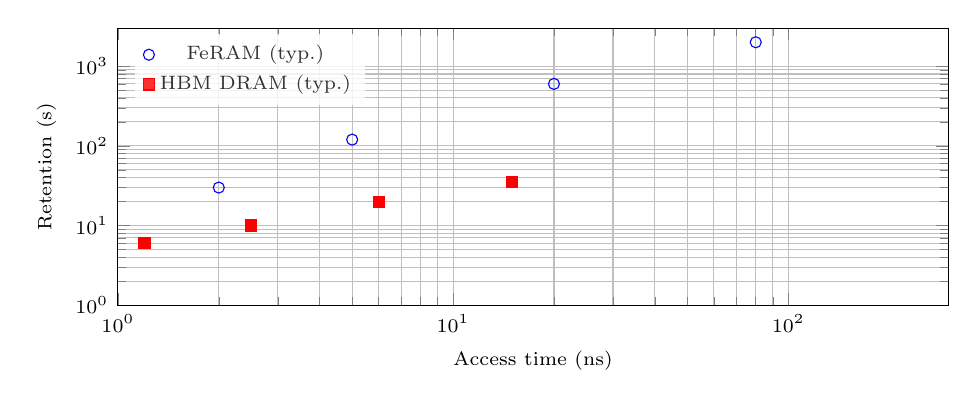
\begin{tikzpicture}
\begin{loglogaxis}[
  width=\columnwidth, height=5.1cm,
  xmin=1e0, xmax=3e2, ymin=1e0, ymax=3e3,
  xlabel={Access time (ns)}, ylabel={Retention (s)},
  grid=both,
  tick label style={font=\scriptsize}, label style={font=\scriptsize},
  legend style={
    at={(0.02,0.98)}, anchor=north west,
    draw=none, fill=white, fill opacity=0.8,
    font=\scriptsize
  }
]
  % FeRAM: blue circles
  \addplot+[only marks, mark=o] coordinates
    {(2,30) (5,120) (20,600) (80,2000)};
  \addlegendentry{FeRAM (typ.)}

  % HBM: red squares
  \addplot+[only marks, mark=square*, mark options={fill=red}] coordinates
    {(1.2,6) (2.5,10) (6,20) (15,35)};
  \addlegendentry{HBM DRAM (typ.)}
\end{loglogaxis}
\end{tikzpicture}
\caption{Access time vs. retention. Red squares: HBM; blue circles: FeRAM. FeRAM extends the retention axis while maintaining feasible access times.}
\label{fig:retention_tradeoff}
\end{figure}
